\iffalse
\let\negmedspace\undefined
\let\negthickspace\undefined
\documentclass[journal,12pt,twocolumn]{IEEEtran}
\usepackage{cite}
\usepackage{amsmath,amssymb,amsfonts,amsthm}
\usepackage{algorithmic}
\usepackage{graphicx}
\usepackage{textcomp}
\usepackage{xcolor}
\usepackage{txfonts}
\usepackage{listings}
\usepackage{enumitem}
\usepackage{mathtools}
\usepackage{gensymb}
\usepackage{comment}
\usepackage[breaklinks=true]{hyperref}
\usepackage{tkz-euclide} 
\usepackage{listings}
\usepackage{gvv}                                        
\def\inputGnumericTable{}                                 
\usepackage[latin1]{inputenc}                                
\usepackage{color}                                            
\usepackage{array}                                            
\usepackage{longtable}                                       
\usepackage{calc}                                             
\usepackage{multirow}                                         
\usepackage{hhline}                                           
\usepackage{ifthen}                                           
\usepackage{lscape}
\newtheorem{theorem}{Theorem}[section]
\newtheorem{problem}{Problem}
\newtheorem{proposition}{Proposition}[section]
\newtheorem{lemma}{Lemma}[section]
\newtheorem{corollary}[theorem]{Corollary}
\newtheorem{example}{Example}[section]
\newtheorem{definition}[problem]{Definition}
\newcommand{\BEQA}{\begin{eqnarray}}
\newcommand{\EEQA}{\end{eqnarray}}
\newcommand{\define}{\stackrel{\triangle}{=}}
\theoremstyle{remark}
\newtheorem{rem}{Remark}
\begin{document}
\parindent 0px
\bibliographystyle{IEEEtran}

\title{Assignment\\[1ex]11.9.5 - 22}
\author{EE23BTECH11220 - R.V.S.S Varun$^{}$% <-this % stops a space
}
\maketitle
\newpage
\bigskip

\renewcommand{\thefigure}{\theenumi}
\renewcommand{\thetable}{\theenumi}
\section*{Question}
Find the 20th term in this series.\\
$$2\times4+4\times6+6\times8\cdots+n\,terms$$ 

\fi


\begin{table}[h]
    \centering
    \begin{tabular}{|p{2cm}|p{2.5cm}|p{2.3cm}|}
    \hline
    PARAMETER & VALUE & DESCRIPTION  \\ \hline
    $$x\brak0$$ & $$8$$ & First term \\ \hline
	$$x(n)$$ & $$4\brak{n+1}{n+2}u\brak n$$ & General term of the series  \\ 
    \hline
  \end{tabular}

    \caption{Table of parameters}
    \label{tab:11.9.5.22.1}
\end{table}


Using $Z$- transform,
\begin{align}
	n^2 u\brak{n}\xleftrightarrow{\mathcal{Z}} \frac{z^{-1}\brak{z^{-1}+1}}{\brak{1-z^{-1}}^3} ,  \abs{z} > 1
\end{align}
\begin{align}
	n u\brak{n}\xleftrightarrow{\mathcal{Z}} \frac{z^{-1}}{\brak{1-z^{-1}}^2} ,   \abs{z} >1 
\end{align}
\begin{align}
	u\brak{n}\xleftrightarrow{\mathcal{Z}} \frac{1}{\brak{1-z^-1}} ,   \abs{z} >1 
\end{align}
\begin{align}
    X\brak{z}=\sum_{n=-\infty}^{n=\infty}4\brak{n+1}\brak{n+2}u\brak{n}z^{-n}
\end{align}
\begin{align}
	X\brak{z}=\sum_{n=-\infty}^{n=\infty}4\brak{n^2+3n+2}u\brak{n}z^{-n}
\end{align}
\begin{align}
	X\brak{z}=\frac{8}{\brak{1-z^{-1}}^3} , \abs{z} >1\\
	y\brak{n}&=x\brak{n}\ast u\brak{n}\\
	\implies Y\brak{z}&=X\brak{z}U\brak{z}   \\
	 Y\brak{z}&=\brak{\frac{8}{({1-z^{-1})}^{3}}}\brak{\frac{1}{1-z^{-1}}}  \\
	 &=\frac{8}{({1-z^{-1})}^{4}} ,\quad \abs{z}>1
\end{align}
Using Contour Integration to find the inverse $Z$-transform,
\begin{align}
    y(19)&=\frac{1}{2\pi j}\oint_{C}Y(z) \;z^{18} \;dz  \\
    &=\frac{1}{2\pi j}\oint_{C}\frac{8z^{18}}{({1-z^{-1})}^{4}} \;dz 
\end{align}
We can observe that the pole is repeated $4$ times and thus $m=4$,
\begin{align}
    R&=\frac{1}{\brak {m-1}!}\lim\limits_{z\to a}\frac{d^{m-1}}{dz^{m-1}}\brak {{(z-a)}^{m}f\brak z}  \\
    &=\frac{1}{\brak {3}!}\lim\limits_{z\to 1}\frac{d^{3}}{dz^{3}}\brak {{(z-1)}^{4}\frac{8z^{22}}{{(z-1)}^4}}   \\
	&=\frac{4}{3}\lim\limits_{z\to 1}\frac{d^3}{dz^3}(z^{22})   \\
    &=12320
\end{align}
\begin{align}
    \therefore \boxed{y(19)=12320}
\end{align}

\begin{figure}[ht]
    \centering
	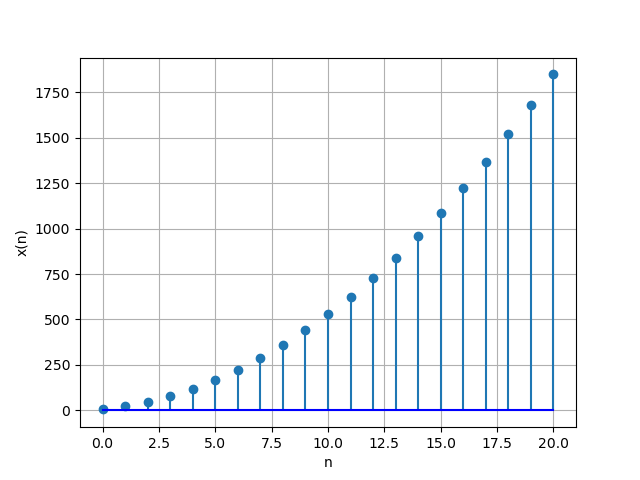
\includegraphics[width=1\columnwidth]{ncert-maths/11/9/5/22/graphs/digital2_graph.png}
    
	\label{fig:11.9.5.22.1}
\end{figure}
